\section{A basic proof of the Higgs mechanism}
\label{sec:higgs_proof}
In what follows we will go over the Higgs mechanism. A lot of this section is beyond the scope of what
you need to know for the exam. However you might find it interesting to see where the ideas come from
in a non-technical way, giving you a feeling of the 
process with which the $W$ and $Z$ bosons obtain mass, also known as the ``Higgs mechanism''. We will also see the impact this has on how fundamental fermions obtain mass, what the Higgs boson is and how it was discovered. Next year, armed with the weapons of field theory, together with a bit of group theory you will see the full beauty of this mechanism.

\subsection{Towards gauge invariance}

There are laws in physics which are not sensitive
to the absolute values of physical quantities but rather to their size relative to particular choice of a baseline. 

Consider for example potential energy. Typically in a mechanics problem you have the freedom to choose where the zero potential is. That is, your laws of physics remain unchanged under the shifting of your potential energy:\[V\to V+C\] where $C$ is some constant, because what matters is the potential difference, $\Delta V$, rather than the absolute value of $V$.

Another example of this freedom, can be found in electro-magnetism and Maxwell's equations written in terms of the magnetic vector potential $\vec{A}$ and the electric potential $\phi$. One can basically pick any scalar function, lets call this $\lambda$, such we can then transform $\vec{A}$ and $\phi$ according to:
\begin{eqnarray}
\label{eq:gauge_transformation}
\vec{A'}=\vec{A}+\nabla\lambda\\
\phi'=\phi-\frac{\partial\lambda}{\partial t}\notag
\end{eqnarray}
Such a transformation, typically called a ``gauge transformation'' would leave the form of Maxwell's equations in terms of $\vec{E}$ and $\vec{B}$ invariant. Therefore one can pick forms of $\lambda$ to simplify Maxwell's equations depending on the problem one needs to solve. For example, one choice of $\lambda$ is such that it allows one to write
\[
\nabla\cdot\vec{A}+\frac{1}{c^2}\frac{\partial\phi}{\partial t}=0
\]
and is called the Lorenz gauge (anyway this last bit is not important but I hope it rings the bell from your EM courses)

\subsection{Masses of $W$ and $Z$ bosons}
So what on earth does all this have to do with how one gives masses to the $W$ and the $Z$? First of all let me remind you that the $W$ and the $Z$ are special because they are the only ``force carriers'' in the Standard Model of particle physics that have mass. The photon and the gluon are massless. As the $W$ and $Z$ are force carriers they have spin 1 and thus can be thought of as massive versions of the photon. Thus one could write down a theory of weak interactions in complete analogy to Maxwell's equation, but with the addition of a mass term. How should this mass term look like? Well we can take inspiration from the Klein-Gordon equation, Eq.~\ref{eq:klein_gordon}, remembering that we need to have a relativistic equation that satisfies $E^2=p^2+m^2$. All in all we can therefore write:
\begin{eqnarray}
\nabla^{2}\vec{A}_{W,Z}-\frac{\partial^2\vec{A}_{W,Z}}{\partial^2t}+m_{W,Z}^2\vec{A}_{W,Z}=0\\
\nabla^{2}\phi_{W,Z}-\frac{\partial^2\phi_{W,Z}}{\partial^2t}+m_{W,Z}^2 \phi_{W,Z}=0
\end{eqnarray}
where $\vec{A}_{W,Z}$ and $\phi_{W,Z}$ are the magnetic vector and electric scalar potentials for the $W$ and $Z$ bosons respectively, and $m_{W,Z}$ are the $W$ and $Z$ masses.
Note we have used natural units and have written the form of Maxwell's equation in the vacuum. 

We can write the above equation a bit more neatly by noting that $\vec{A}$ and $\phi$ can be combined in a form of a four-vector $\mathcal{A}=(\phi,\vec{A})$. We therefore have:
\begin{equation}
\label{eq:proca}
\nabla^{2}\mathcal{A}_{W,Z}-\frac{\partial^2\mathcal{A}_{W,Z}}{\partial^2t}+m_{W,Z}^2\mathcal{A}_{W,Z}=0\\
\end{equation}
The above equation is known as the ``Proca-equation'' and it represents the equivalent of Maxwell's equation for a massive field. This is a bit of a simplification, as the $W$ and $Z$ bosons contain weak charge and thus, in contrast to the photon, they self-interact (similar to the gluon). Nevertheless Eq.~\ref{eq:proca} acts as a good educational example.

Now there is a major problem with Eq.~\ref{eq:proca}. It turns out that if one performs a gauge transformation for $\vec{A}_{W,Z}$ and $\phi_{W,Z}$ along the lines of Eq.~\ref{eq:gauge_transformation}, the presence of the mass term means that Eq.~\ref{eq:proca} is not invariant! Invariance under a gauge transformation as you shall see next year is an extremely important requirement in nature and therefore adding a mass term
in this simplistic way is an absolute failure!!

\subsection{Masses of electrons (fermions)}
One of the outcomes of the Dirac equation, Eq.~\ref{eq:dirac_equation}, is that it tells us that a left handed fermion (e.g an electron) can convert into a right handed fermion as it moves in space and time. The rate at which this effect occurs is determined by mass of the fermion. 

Consider the couplings of fermions like quarks or electrons to the $Z^0$ boson. Just like why an electrically charged object can interact with the photon,  fermions interact with a $Z^0$ boson because they carry an analogous type of charge, called the weak hypercharge. Just as electric charge, weak hypercharge is a conserved quantity.
The Standard Model of particle physics however, has the peculiarity that left handed electrons have 1 unit of weak hypercharge, but right handed electrons have 0 weak hypercharge. This means that the transition of a left handed electron to a right handed electron, whose rate is related to the electron mass, violates conservation of weak hypercharge! Oh dear. This means that in the Standard Model, all fermions must be massless in order to conserve weak hypercharge! So what on earth do we do now that everything seems broken? We could huddle in a corner and cry...

\subsection{Enter the Higgs}
In order to be able to write down an equation for massive force carriers as well as massive fermions, we need to introduce a complex field $\Phi$ which is always turned on. That is, even in the ground state of the universe this field exists, ie the (expectation) value of this field even in the vacuum is non-zero. 
The figures below give examples of the potential energies fields as a function of the field strength itself. The figure on the left is for a field whose value at the vacuum (minimum potential energy) is zero, just like the EM field (though the EM field is real not complex). The example on the right corresponds to this new field $\Phi$ we need to introduce.
\begin{center}
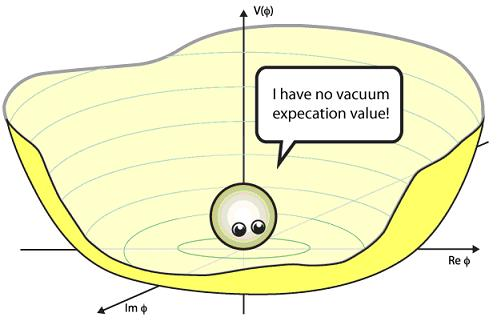
\includegraphics[width=0.45\textwidth]{fig/higgs/phi_stable.JPG}
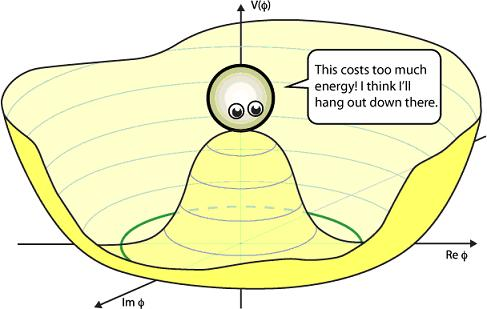
\includegraphics[width=0.45\textwidth]{fig/higgs/phi_unstable.JPG}
\end{center}

Before we continue we need to upgrade our understanding of how fields and particles are connected.
\paragraph{Basic principle of Quantum Field Theory}
We can think of a field at a point in space and time as a little ball which we can excite by imparting energy away from the minimum of the potential energy of the field. So we can displace the field from the minimum and set it to rotate around an equipotential as shown in the figure below. 
\begin{center}
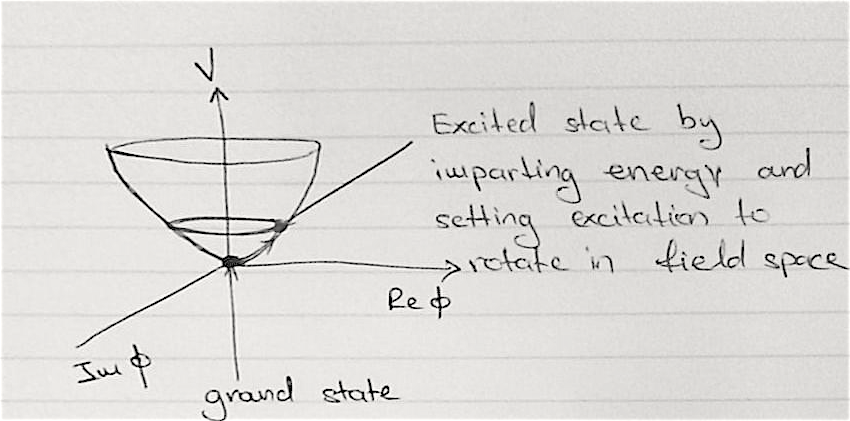
\includegraphics[width=0.85\textwidth]{fig/higgs/field_excitation_bw.png}
\end{center}
The little ball now obtains some angular momentum but not in the typical sense of angular momentum, as the rotation is not in normal space, but in this (internal) field space. In fact just as angular momentum in QM, this special angular momentum is also quantised and it corresponds to another quantum number, charge! {\bf In other words, in modern physics (Quantum Field Theory) we think of a charged particle as an excitation of the field in which this excitation is made to rotate around the internal space of the field.}

Lets go back to the case where the potential of the $\Phi$ field whose field value at the minimum is non-zero. This means that we do not need to impart any energy to create an excitation of the field (a particle), as the field is already non-zero. Thus by imparting an infinitesimally small amount of energy to the particle, we can set the particle to rotate around the minimum as shown in the figure below, thus creating a ``charged'' particle. 
\begin{center}
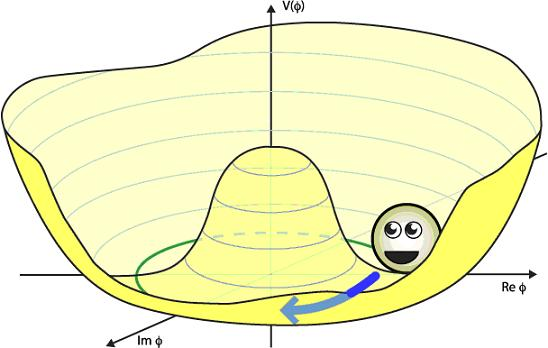
\includegraphics[width=0.85\textwidth]{fig/higgs/phi_goldstone.JPG}
\end{center}
Note  that there is no physical requirement that stops us from having a field always turned on. So for each point in space and time we can setup such a rotation and produce a set of charged particles at a cost of no energy. Such a phenomenon is called ``Condensate of charge in space''. Now the true ground state of this condensate would be one where there is no rotation or no charge. But the uncertainty principle tells us that we cannot have a state exactly localised in space with exactly no momentum.
\[
\Delta x\Delta p\geq\hbar
\]
Thus we cannot create a bunch of particles at exactly known positions without any total ``charge'' because if we know $x$ exactly then there is an equal probability of finding a particle with any momentum $p$. Therefore the condensate is a strange configuration of space where there is a non zero amount of charge its value is completely uncertain!! The upshot of this is that adding or removing  units of charge, does not change the total charge of the system as the charge is unknown!!  {\bf NOTE electric charge is not the same. However materials such as super-conductors behave as such!!}

\subsection{Resolution of fermion masses}
Lets go back to consider a massive electron (fermion) which is flipping between a left handed and right handed state. As long as weak hypercharge is conserved, then electrons are allowed to have mass. We can therefore explain massive fermions by requiring that they are constantly depositing/withdrawing a unit of hyper-charge to this $\Phi$ condensate whose rotational excitations are denoted as $\phi$ and we require that this $\phi$ carries a weak hypercharge of 1. Since the charge of the condensate is utterly unknown, as argued through the uncertainty principle, we are free to add or remove units of weak hypercharge to/from the condensate at no cost. The figure below gives more details
\begin{center}
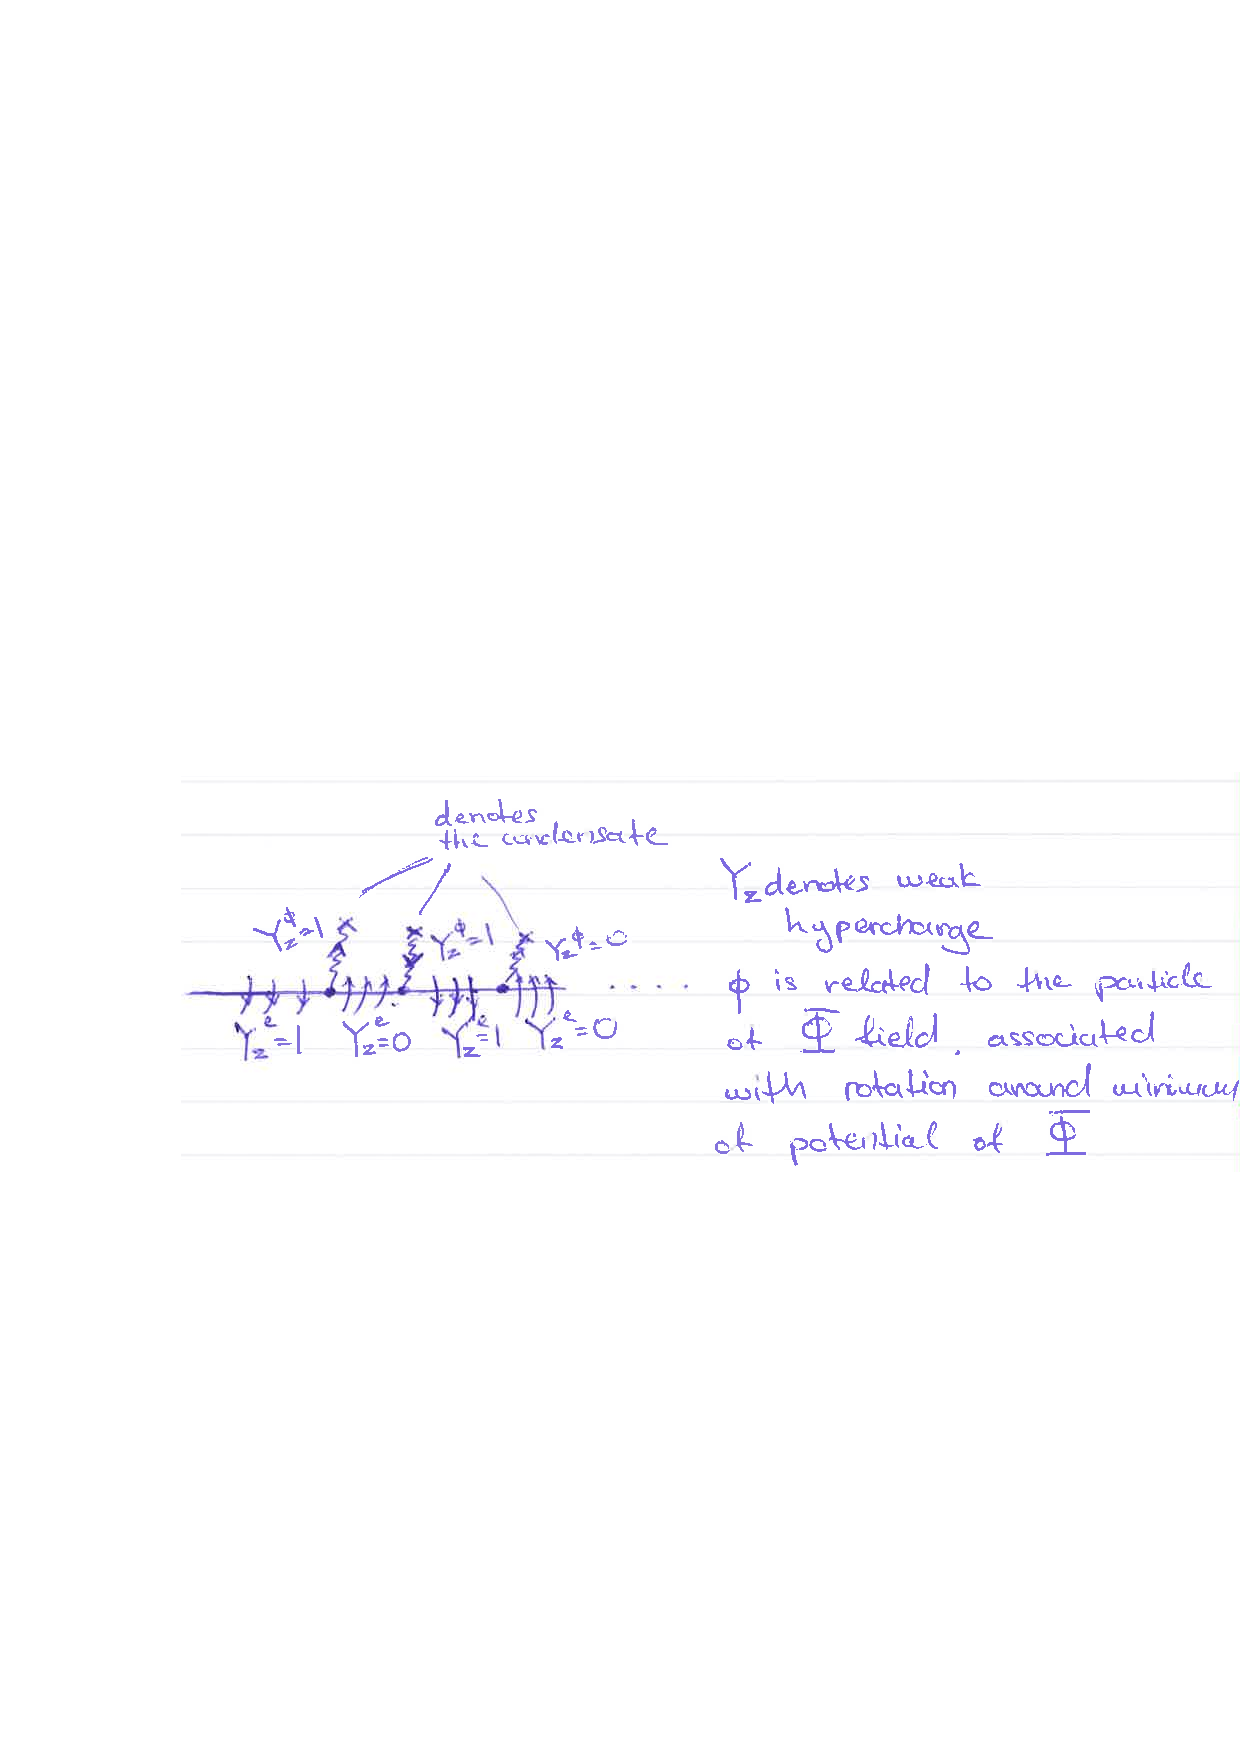
\includegraphics[width=0.95\textwidth]{fig/higgs/fermion_mass.pdf}
\end{center}

\subsection{Resolution of $Z^0$ and $W$ masses}
Similarly the interaction of the $Z^0$ and $W$ with the condensate field $\phi$ gives rise to their masses (strength of the interaction related to the $Z^0$ boson mass). The figure below gives more detail.
\begin{center}
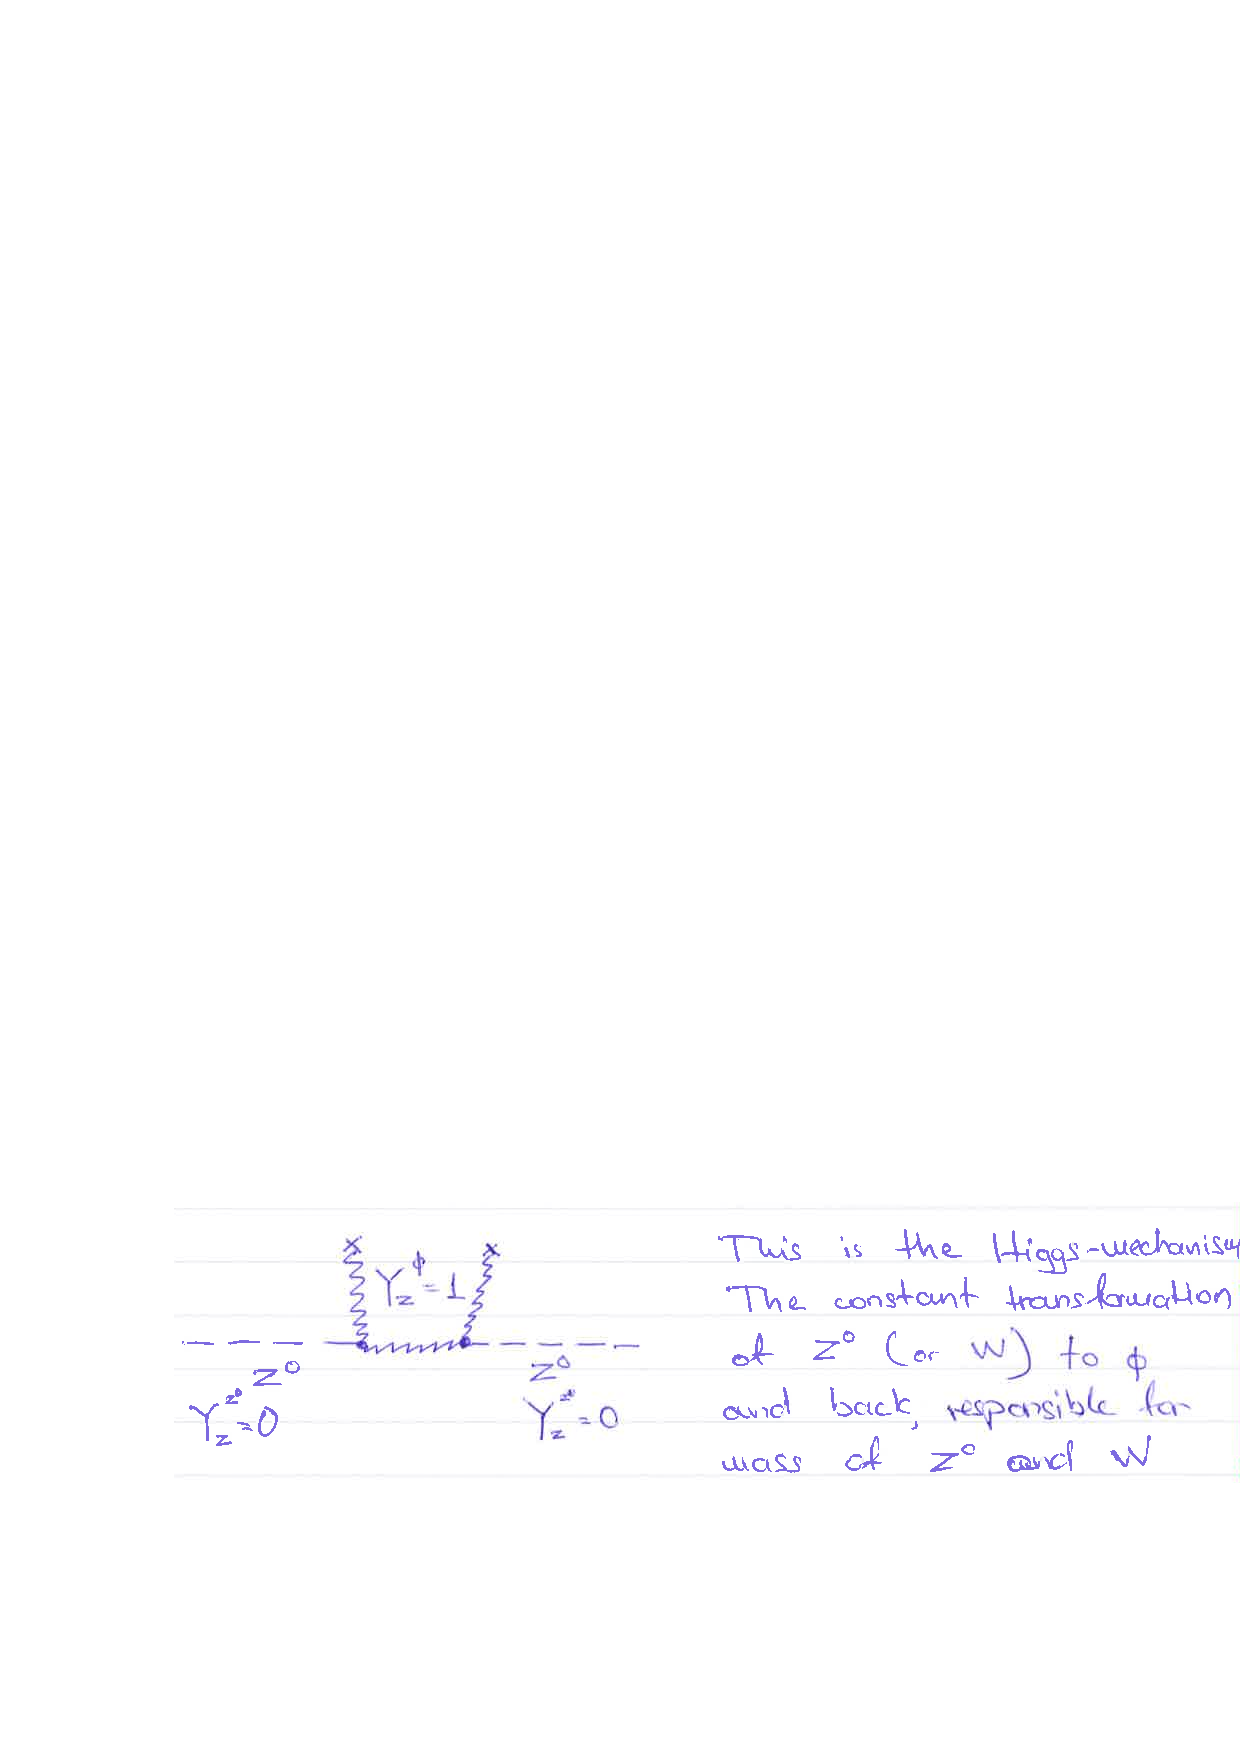
\includegraphics[width=0.95\textwidth]{fig/higgs/boson_mass.pdf}
\end{center}

\subsection{Right, what about the Higgs boson?}
Ok so I have been dancing around the point a bit. $\Phi$ and $\phi$, although related to the Higgs boson, strictly speaking are NOT the Higgs boson (could have guessed by the fact I have not called them $H$ or $h$). The Higgs boson, lets call it $H$, is a different excitation mode than the $\phi$. Instead of kicking ``circularly'' around the minimum, you impart some energy along the slope of the potential. This so called radial excitation, is the Higgs boson. 
\begin{center}
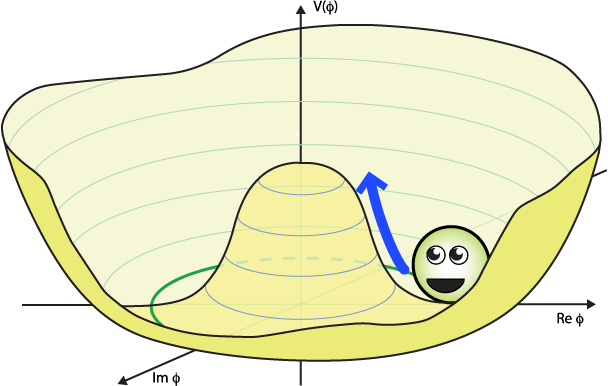
\includegraphics[width=0.95\textwidth]{fig/higgs/phi_higgs.png}
\end{center}

In fact the particle $\phi$ turns out is an unphysical state which gets absorbed by the $Z^0$ when the $Z^0$ obtains its mass. Think of it like this. Before the $Z^0$ obtains mass, the $Z^0$ has 2 degrees of freedom corresponding to the two polarisations just like the photon. The $\phi$ acts as a third degree of freedom. As soon as the $Z^0$ boson obtains mass, it obtains an additional longitudinal polarisation. This additional degree of freedom arises when the state $\phi$ gets ``eaten up'' by the $Z^0$ boson thus allowing the $Z^0$ to obtains its mass. Therefore, the system overall still retains 3 degrees of freedom\footnote{Much more about this next year}! 

{\bf The coupling strength of the Higgs boson to other particles, is proportional to the mass of the particle the Higgs couples to. So the probability that a Higgs will decay to a particular particle is proportional to the mass of the particle the Higgs couples to squared.}
Recent measurements seem to verify this fact as the figure below suggests. The y-axis is the coupling strength, the x-axis is the mass of the particle the Higgs decayed to.
\begin{center}
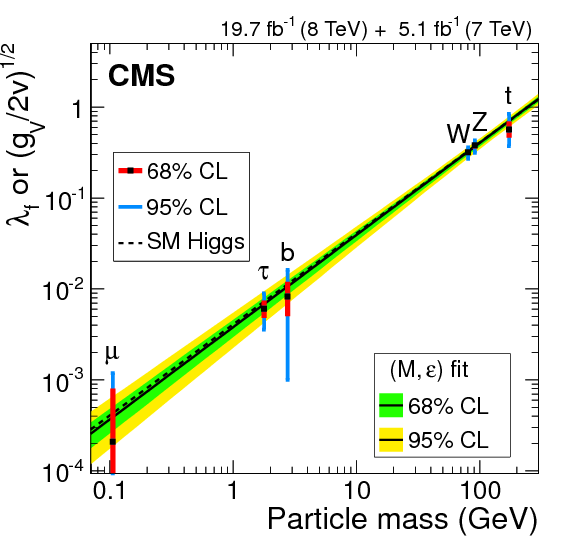
\includegraphics[width=0.95\textwidth]{fig/higgs/cms_higgs_couplings.png}
\end{center}

